\documentclass[12pt,a4paper]{article}
\usepackage{rmpackages}																% usual packages
\usepackage{rmtemplate}																% graphic charter
\usepackage{rmexocptce}																% for DS with cptce eval

%\cfoot{} 													% if no page number is needed
%\renewcommand\arraystretch{1.5}		% stretch table line height

\newcommand{\ritem}{\refstepcounter{enumi}\item[\writeit{} \theenumi .]}

\begin{document}

\begin{header}
TP -- La tête dans les étoiles
\end{header}

\begin{multicols}{2}
\begin{center}
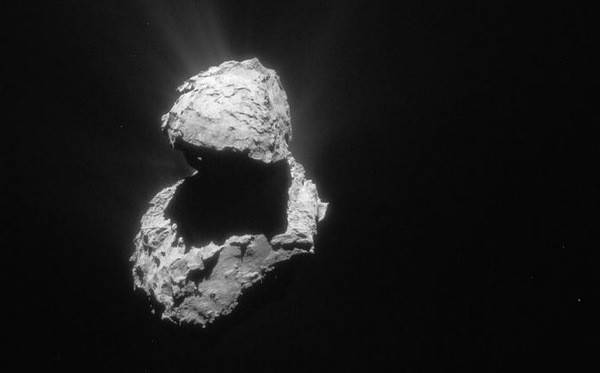
\includegraphics[width=\linewidth]{images/tchouri3.jpg}
\end{center}

En 2014, après dix années de voyage à bord de la sonde européenne Rosetta, le module Philae atteignait enfin sa destination : une comète surnommée \og Tchouri \fg{}.
Première à réaliser l'exploit de se poser à la surface d'une comète, Philae a pu récolter des données qui aident la communauté scientifique à comprendre les processus de formation du système solaire.
La comète Tchouri repassera à proximité de la Terre à la fin de cette année 2021, sans toutefois la menacer.
\end{multicols}

L'objectif de ce TP est d'étudier la trajectoire de quelques objets du système solaire en utilisant Python et les relevés de position effectués par des astrophysiciens.

\begin{enumerate}
\item \rea{}

Copier-coller tout le dossier \og TP Tchouri \fg{} dans votre espace de travail personnel (Ordinateur \textrightarrow{} Ma classe \textrightarrow{} Documents en consultation \textrightarrow{} Physique-Chimie \textrightarrow{} TP Tchouri).
\end{enumerate}

\section*{Organisation des données}

\begin{enumerate}[resume]
\ritem \app{}

Ouvrir le fichier \texttt{earth.txt} avec Notepad++.
À quoi correspondent les valeurs contenues dans chacune des deux colonnes à partir de la ligne 8 ?
Quelle est l'unité de ces valeurs ?
% Lisez les informations de l'entête du fichier.
% Une unité astronomique permet d'exprimer une durée, une vitesse, une distance ?

\ritem \app{}

Donner l'intervalle de temps qui sépare les valeurs de deux lignes consécutives.
% Lisez l'entête !
% On aurait pu rajouter une colonne devant les positions XY qui indique le temps écoulé depuis la première position. Quelles valeurs aurait-on mis dans cette colonne ?

\ritem \app{} \anarai{} \rea{}

%Exprimer en années la durée sur laquelle s'étalent les données de l'ensemble du fichier.
À un mois près, à quelle date correspond la dernière ligne du document ?
% Combien de jours séparent la première ligne de la deuxième ? De la troisième ? ... De la dernière ?
% Combien y a-t-il de lignes dans le fichier ?
\end{enumerate}

\section*{Première trajectoire : la Terre}

\begin{enumerate}[resume]
\ritem \rea{} \app{}

Ouvrir le programme \texttt{position\_planetes.py} avec EduPython et l'exécuter 
\includegraphics[height=0.75\baselineskip]{images/edupython_execute.png}.
Décrire ce qui est représenté sur le graphe.

\ritem \app{}

Par rapport à quoi sont représentées les positions de la Terre ?
% Quelle est l'origine du repère ?

\ritem \app{} \anarai{}

Proposer une hypothèse sur la signification des deux paramètres de l'étude \texttt{nb\_jours} et \texttt{delta\_jours} des lignes 19 et 22.

\ritem \anarai{} \rea{} \val{}

Proposer un protocole permettant de vérifier votre hypothèse, puis la vérifier.
\end{enumerate}
\begin{appel}
\anarai{}
\end{appel}
\newpage

\begin{enumerate}[resume]
\item \anarai{} \val{}

Modifier le programme pour représenter un nombre \textbf{suffisant mais pas trop élevé} de positions successives de la Terre pendant \textbf{une} révolution complète autour du Soleil pour bien décrire sa trajectoire et de manière à ce que l'intervalle entre deux positions successives reste bien visible.
% Combien de jours faut-il à la Terre pour faire un tour autour du Soleil ? 
% Elle tourne dans quel sens la Terre ?
\end{enumerate}
\begin{appel}
\val{}
\end{appel}

\begin{enumerate}[resume]
\ritem \rco{}

Choisir parmi les mots suivants ceux qui permettent de caractériser le mouvement de la Terre autour du Soleil : rectiligne, circulaire, curviligne, uniforme, accéléré, décéléré.
\end{enumerate}

\section*{Elle est passée par ici, elle repassera par là}

\begin{enumerate}[resume]

\ritem \app{} \anarai{}

Quel est le rôle de la commande \texttt{plt.plot} ligne 46 ?

\item \anarai{}

Modifier le programme ligne 49 pour afficher aussi les positions successives de la comète Tchouri.

\ritem \app{} \anarai{} \val{}

Donner le numéro des lignes du programme permettant de modifier les limites du graphe. 
Modifier le programme pour visualiser l'ensemble des positions de Tchouri.

\ritem \anarai{} \rea{} \val{}

Déterminer la période de la comète Tchouri, c'est à dire la durée nécessaire pour qu'elle effectue un tour complet autour du soleil.
\end{enumerate}

\begin{appel}
\rea{}
\end{appel}

\end{document}